\section{Auswahl der Technologie - Client}
\setauthor{David Hauser}

\subsection{Unterschied Framework und Library}
\subsection{Technologie zur Entwicklung des Frontends}
\subsection{Angular}
\subsection{React}

\section{Auswahl der Technologie - Datenbank[SK]}
\setauthor{Simon Koll}
Die Datenbank spielt für das Projekt eine wichtige Rolle, daher wurden hier folgende Kriterien aufgestellt:

\begin{itemize}
  \item Das Projekt besteht aus Hard- und Software, die Daten sowohl abspeichern als auch abfragen. Das kann je nach Anwendungsfall unterschiedlich sein.
  \item Vom Dashboard können beispielsweise Kennzeichen mit Gültigkeitsdauer, aber auch nur einfache NFC-Codes gesendet werden.
  \item In der Zukunft soll die Möglichkeit bestehen, weitere Zutrittsmöglichkeit hinzuzufügen. Daher muss sich die Datenbank der sich ändernden Datenstruktur anpassen können.
\end{itemize}

\subsection{Relationale Datenbanken}

Das Team befand sich nun vor der Entscheidung, ein relationales Datenbanksystem zu verwenden, oder ein nicht relationales Datenbanksystem.
Die größten Unterschiede hierbei sind, dass bei relationalen SQL-Datenbanken den gespeicherten Daten Tabellen vorgegeben sind, das sogenannte Schema. Das ist bei NoSQL-Datenbanken ebenfalls möglich, jedoch optional.
Relationale Datenbanken verfolgen das ACID-Prinzip. ACID steht für

\begin{itemize}
  \item \textit{Atomicity}
  \subitem Alle Änderungen der Datenbank werden als einzige Operation verarbeitet. Entweder werden alle Änderungen wie Inserts, Updates usw. durchgeführt, oder keine davon.
  \item \textit{Consistency}
  \subitem Zu Beginn und zum Ende jeder Transaktion sind die Daten konsistent.Beispielsweise bei einer Geldüberweisung, ist bei "Consistency" die Gesamtsumme der Geldmittel auf beiden Konten am Anfang und am Ende jeder Transaktion gleich.
  \item \textit{Isolation}
  \subitem Andere Transaktionen haben keine Einsicht in die Transaktion. Isolation bedeutet also, dass parallel laufende Transaktionen sich wie serialisierte verhalten.
  \item \textit{Durability}
  \subitem Die Daten bleiben nach Ende der Transaktion bestehen und auch bei einem kompletten Systemausfall nicht revidiert.
\end{itemize}
\cite{ACID}

\subsection{MongoDB}
Das Team entschied sich für eine der bekanntesten NoSQL-Datenbanken, \textbf{MongoDB}. Diese bietet einige Vorteile gegenüber den relationalen SQL-Datenbanken:

\begin{itemize}
  \item \textit{Skalierbarkeit: } MongoDB Datenbanken zeichnen sich durch ihre ausgezeichnete horizontale Skalierbarkeit aus. Horizontale Skalierbarkeit bedeutet, dass die Datenbank sich problemlos über mehrere Server verteilen kann, ohne die Funktionsfähigkeiten zu beeinträchtigen.
  \item \textit{Verfügbarkeit}
  \item \textit{Flexibilität}
\end{itemize}
\cite{VorteileMongoDB}
\section{Auswahl der Technologie - Kennzeichenerkennung[SK]}
\setauthor{Simon Koll}
Das Herz von APERTA ist die Kennzeichenerkennung. Dieses Alleinstellungsmerkmal separiert das Projekt von möglicher Konkurrenz. Um eine schnelle, und problemfreie Lösung zu liefern, versuchte das Team, eine für österreichische Kennzeichen optimierte Lösung zu implementieren. Dabei spielen Faktoren wie der Aufnahmewinkel der Kamera, die Distanz zum Kennzeichen, sowie die Lichtsituation eine entscheidende Rolle. Weiters muss aus den Einzelbildern der Kamera das Kennzeichen erkannt werden und danach die Buchstaben aus dem Bild extrahiert werden. Um dies zu vollbringen, werden 2 Libraries verwendet.
\subsection{OpenCV: } OpenCV steht für Open Source Computer Vision und ist eine frei Zugängliche Library, welche meist in Bereichen wie Machine Learning oder Machine Vision ihren Einsatz findet. Unternehmen können kostenlos auf die Bibliothek zugreifen, verändern und weiterentwickeln. Die Basis bilden die mehr als 2500 klassischen und neuen Algorithmen für das maschinelle Sehen. Diese haben unterschiedliche Spezialisierungen, wie unter anderem die Erkennung von Gesichtern, Objekten und Kamerabewegungen, die Generierung von 3D-Modellen, Ähnlichkeiten in Bildern zu finden sowie Markierungen in Augmented Reality anzuzeigen. Zu den mehr als 18 Millionen Downloads und mehr als 47.000 Benutzer:innen zählen meist Unternehmen, Forschungsgruppen oder Regierungsstellen. Bekannte Namen hier sind Google, Microsoft, Intel oder Sony.\cite{AboutOpenCV}
OpenCV hat eine modulare Struktur, was bedeutet, dass das Paket mehrere gemeinsam genutzte oder statische Bibliotheken enthält. Die folgenden Module sind verfügbar:
\begin{itemize}
    \item Kernfunktionalität (core) - ein kompaktes Modul, das grundlegende Datenstrukturen definiert, darunter das dichte mehrdimensionale Array Mat und grundlegende Funktionen, die von allen anderen Modulen verwendet werden.
    \item Bildverarbeitung (imgproc) - ein Bildverarbeitungsmodul, das lineare und nichtlineare Bildfilterung, geometrische Bildtransformationen (Größenänderung, affines und perspektivisches Warping, generisches tabellenbasiertes Remapping), Farbraumkonvertierung, Histogramme usw. umfasst.
    \item Videoanalyse (Video) - ein Videoanalysemodul, das Algorithmen zur Bewegungsschätzung, Hintergrundsubtraktion und Objektverfolgung umfasst.
    \item Kamerakalibrierung und 3D-Rekonstruktion (calib3d) - grundlegende Geometriealgorithmen für mehrere Ansichten, Einzel- und Stereokamerakalibrierung, Objektposenschätzung, Stereokorrespondenzalgorithmen und Elemente der 3D-Rekonstruktion.
    \item 2D Features Framework (features2d) - Erkennung auffälliger Merkmale, Deskriptoren und Deskriptor-Matcher.
    \item Objekterkennung (objdetect) - Erkennung von Objekten und Instanzen der vordefinierten Klassen (z. B. Gesichter, Augen, Tassen, Menschen, Autos usw.).
    \item High-Level-GUI (highgui) - eine leicht zu bedienende Schnittstelle zu einfachen UI-Funktionen.
    \item Video I/O (videoio) - eine einfach zu bedienende Schnittstelle für Videoaufnahmen und Videocodecs.
    \item Einige andere Hilfsmodule, wie z.B. FLANN- und Google-Test-Wrapper, Python-Bindings, und andere.
\end{itemize}
 \subsection{Tesseract: } Tesseract ist eine Texterkennungs-Engine welche von Google entwickelt wird. 

 Optische Zeichenerkennung oder Optical Character Reading (OCR) ist die elektronische oder mechanische Umwandlung von Bildern mit getipptem, handgeschriebenem oder gedrucktem Text in maschinell kodierten Text, sei es aus einem gescannten Dokument, einem Foto eines Dokuments, einem Szenenfoto (z. B. der Text auf Schildern und Werbetafeln in einem Landschaftsfoto) oder aus einem Untertiteltext, der einem Bild überlagert ist (z. B. aus einer Fernsehsendung).
 \cite{ocrWiki}

Um besser zu verstehen, wie OCR funktioniert, hilft dieses Prozessdiagramm in der folgenden Abbildung. Aus Sicht von Endbenutzer:innen ist der OCR-Prozess einfach: Er verarbeitet das Bild und erhält den bearbeitbaren Text.
\begin{figure}[H]
  \centering
  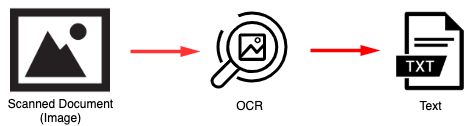
\includegraphics[width=10cm]{pics/OCR-Prozessdiagramm.png}
  \caption{Prozessdiagramm der Optische Zeichenerkennung}
  \cite{introToTesseract}
\end{figure}
 Tesseract bietet die Möglichkeit, Text aus Bildern zu extrahieren. Dies kann in vielen verschiedenen Programmiersprachen erfolgen, oder über eine graphische Nutzeroberfläche eines Drittanbieters.\cite{AboutTesseract} Unterstützt wird Tesseract durch einen Python-Wrapper mit dem Namen \textbf{pytesseract}, welcher Bilder wie .jpeg, .png, .gif und viele mehr laden kann, sowie den gelesenen Text ausgeben kann anstatt ihn in einer Datei abspeichern zu müssen.\cite{AboutPyTesseract}
 
\section{Auswahl der Technologie - Backend[SK]}
\setauthor{Simon Koll}
\subsection{Anforderungen an das Backend}
Für das Backend kamen mehrere Technologien in Frage, wie unter anderem Java, JavaScript, Python, PHP, C$\sharp$, und viele mehr.
Um das Backend zu realisieren, muss die Technologie einige bestimmte Eigenschaften besitzen.\cite{CompareBackendLanguage}
\begin{itemize}
    \item \textit{Java:}
    \subitem Die Vorteile von Java liegen in der Fehlerbehandlung, sowie in Bereichen wie Multithreading und Performanz. Die strikte Fehlerbehandlung führt dabei aber zum Verlust von Flexibilität und Kompaktheit des Codes.
    \item \textit{JavaScript:}
    \subitem Die Syntax von JavaScript ähnelt der von Java. Entwickelt als Scripting-Sprache für HTML, ist JavaScript einfach zu lernen und zu benutzen. Bei der Entwicklung von Websites kann JavaScript direkt in den Quellcode der HTML-Seite eingearbeitet werden. Aber auch im Backend-Bereich kann mit NodeJS in JavaScript entwickelt werden.
    \item \textit{Python:}
    \subitem Python ist eine der mit Abstand am leichtesten zu lesenden Programmiersprachen. Die flache Hierarchie ermöglicht ein einfaches Verständnis von Programmen und Codestücken. Weiters macht Python Entwickler:innen auf Fehler aufmerksam, wenn dieser nicht ausdrücklich ignoriert werden soll.
    Jedoch ist Python manchmal langsamer in der Ausführung als die konkurrierenden Sprachen. Zusätzlich ist durch die Verwendung von Leerzeichen zur Einrückung ein häufiger Fehlergrund hinzugekommen.
    \item \textit{PHP:}
    \subitem Die PHP Syntax erinnert an eine Mischung aus C, Java und Perl. Das Ziel von PHP ist es, Entwickler:innen schnell und einfach dynamisch generierte Webpages zu bauen. Die vermischte Syntax ist jedoch etwas chaotisch, darum ist es leicht sich in falschen Angewohnheiten zu verirren und Sicherheitslücken offen zu lassen.
  \end{itemize}
  Aufgrund vorhandener Vorkenntnisse standen für das Team 3 der oben genannten Technologien zur Auswahl:

  \begin{itemize}
    \item Java,
    \item JavaScript und
    \item Python
  \end{itemize}

  \subsection{Verwendung von NodeJS}
  Von diesen konnte sich JavaScript durchsetzen. Die Gründe dafür waren:\cite{WhyNodeJs}
  \begin{itemize}
    \item NPM:
    Der NPM oder \textit{Node Package Manager}, ist ein Paketmanager für JavaScript, welcher bei NodeJS standardmäßig mitgeliefert wird. Bei NPM werden wiederverwendbare Programmteilen veröffentlicht. Diese können mittels des NPM eingenen Command Line Interfaces installiert werden. Weiters bietet der NPM eine integrierte Versionsverwaltung der Pakete sowie eine Verwaltung der Abhängigkeiten.
    In diesem Projekt wurden beispielsweise die Module \textit{express} und \textit{mongodb} verwendet. 
    \linebreak
    \textit{express} ist ein Framework, welches vor allem in NodeJS Projekten verwendet wird. Die Vorteile von Express sind unter anderem die dem Team bereits bekannte Programmiersprache JavaScript, die Unterstützung der Google V8 engine für bessere Performance, die Robustheit bei einer Vielzahl an HTTP-Anfragen, sowie die einfache Einbindung weiterer Module und Drittanbieterapplikationen. \cite{WhyExpress}
    \linebreak
    \linebreak
    \textit{mongodb} stellt Entwickler:innen eine API zur Verfügung, welche die Nutzung einer MongoDB-Datenbank stark vereinfacht.
    \item Verwendung einer NoSQL Datenbank:
    Aufgrund des Formates, mit dem die Daten aus dem Frontend kommen, bat sich eine nicht relationale Datenbank für das Team an. Die dokumentenorientierte Datenbank MongoDB ist bekannt für ihre hohe Verfügbarkeit, sowie die gute Skalierbarkeit.\cite{WhyMongoDB}
    \linebreak
    \item Behandlung von JSON:
    NodeJS zeichnet sich durch seine einfach Verwendung von JSON-Daten aus. Diese können ohne Parsing oder andere Konvertierungen verarbeitet und darauf zugegriffen werden. Dank NodeJS können JSON Objekte mittels REST-API Anfragen direkt für den Client bereitgestellt werden.
    Danke NodeJS kann eine Einfache Verbindung zwischen Frontend-Clients und dem Backend-Server geschaffen werden.
  \end{itemize}

\section{Auswahl der Technologie - Hardware[SK]}
\setauthor{Simon Koll}
\subsection{Anforderungen an die Hardware}
Das Projekt sollte so vielseitig wie möglich, jedoch auch so kompakt wie möglich sein. Dazu musste auf kleine Komponenten gesetzt werden. Diese soll dennoch leistungsfähig genug sein, um jede der drei Zugangsmöglichkeiten parallel zu verwalten.
\subsubsection{Raspberry Pi}
Die Wahl des Herzstückes fiel auf einen Raspberry Pi.
Der Raspberry Pi ist ein vollwertiger Computer, welcher etwas größer als eine Kreditkarte ist. Er besitzt alle bekannten Anschlüsse eines normalgroßen PCs, wie HDMI-Ausgänge für Monitore, USB-Ports für Peripherie wie Maus, Tastatur oder Webcams, sowie einen LAN-Port für eine kabelgebundene Netzwerkverbindung.
Als Betriebssystem des Raspberry Pi wurde das vom Hersteller empfohlene Raspbian OS verwendet. Dieses bietet eine grafische Benutzeroberfläche, sowie die Möglichkeit den Raspberry auch ohne angeschlossenen Monitor betreiben zu können. \cite{WhatIsRaspberryPi}
\begin{figure}[H]
  \centering
  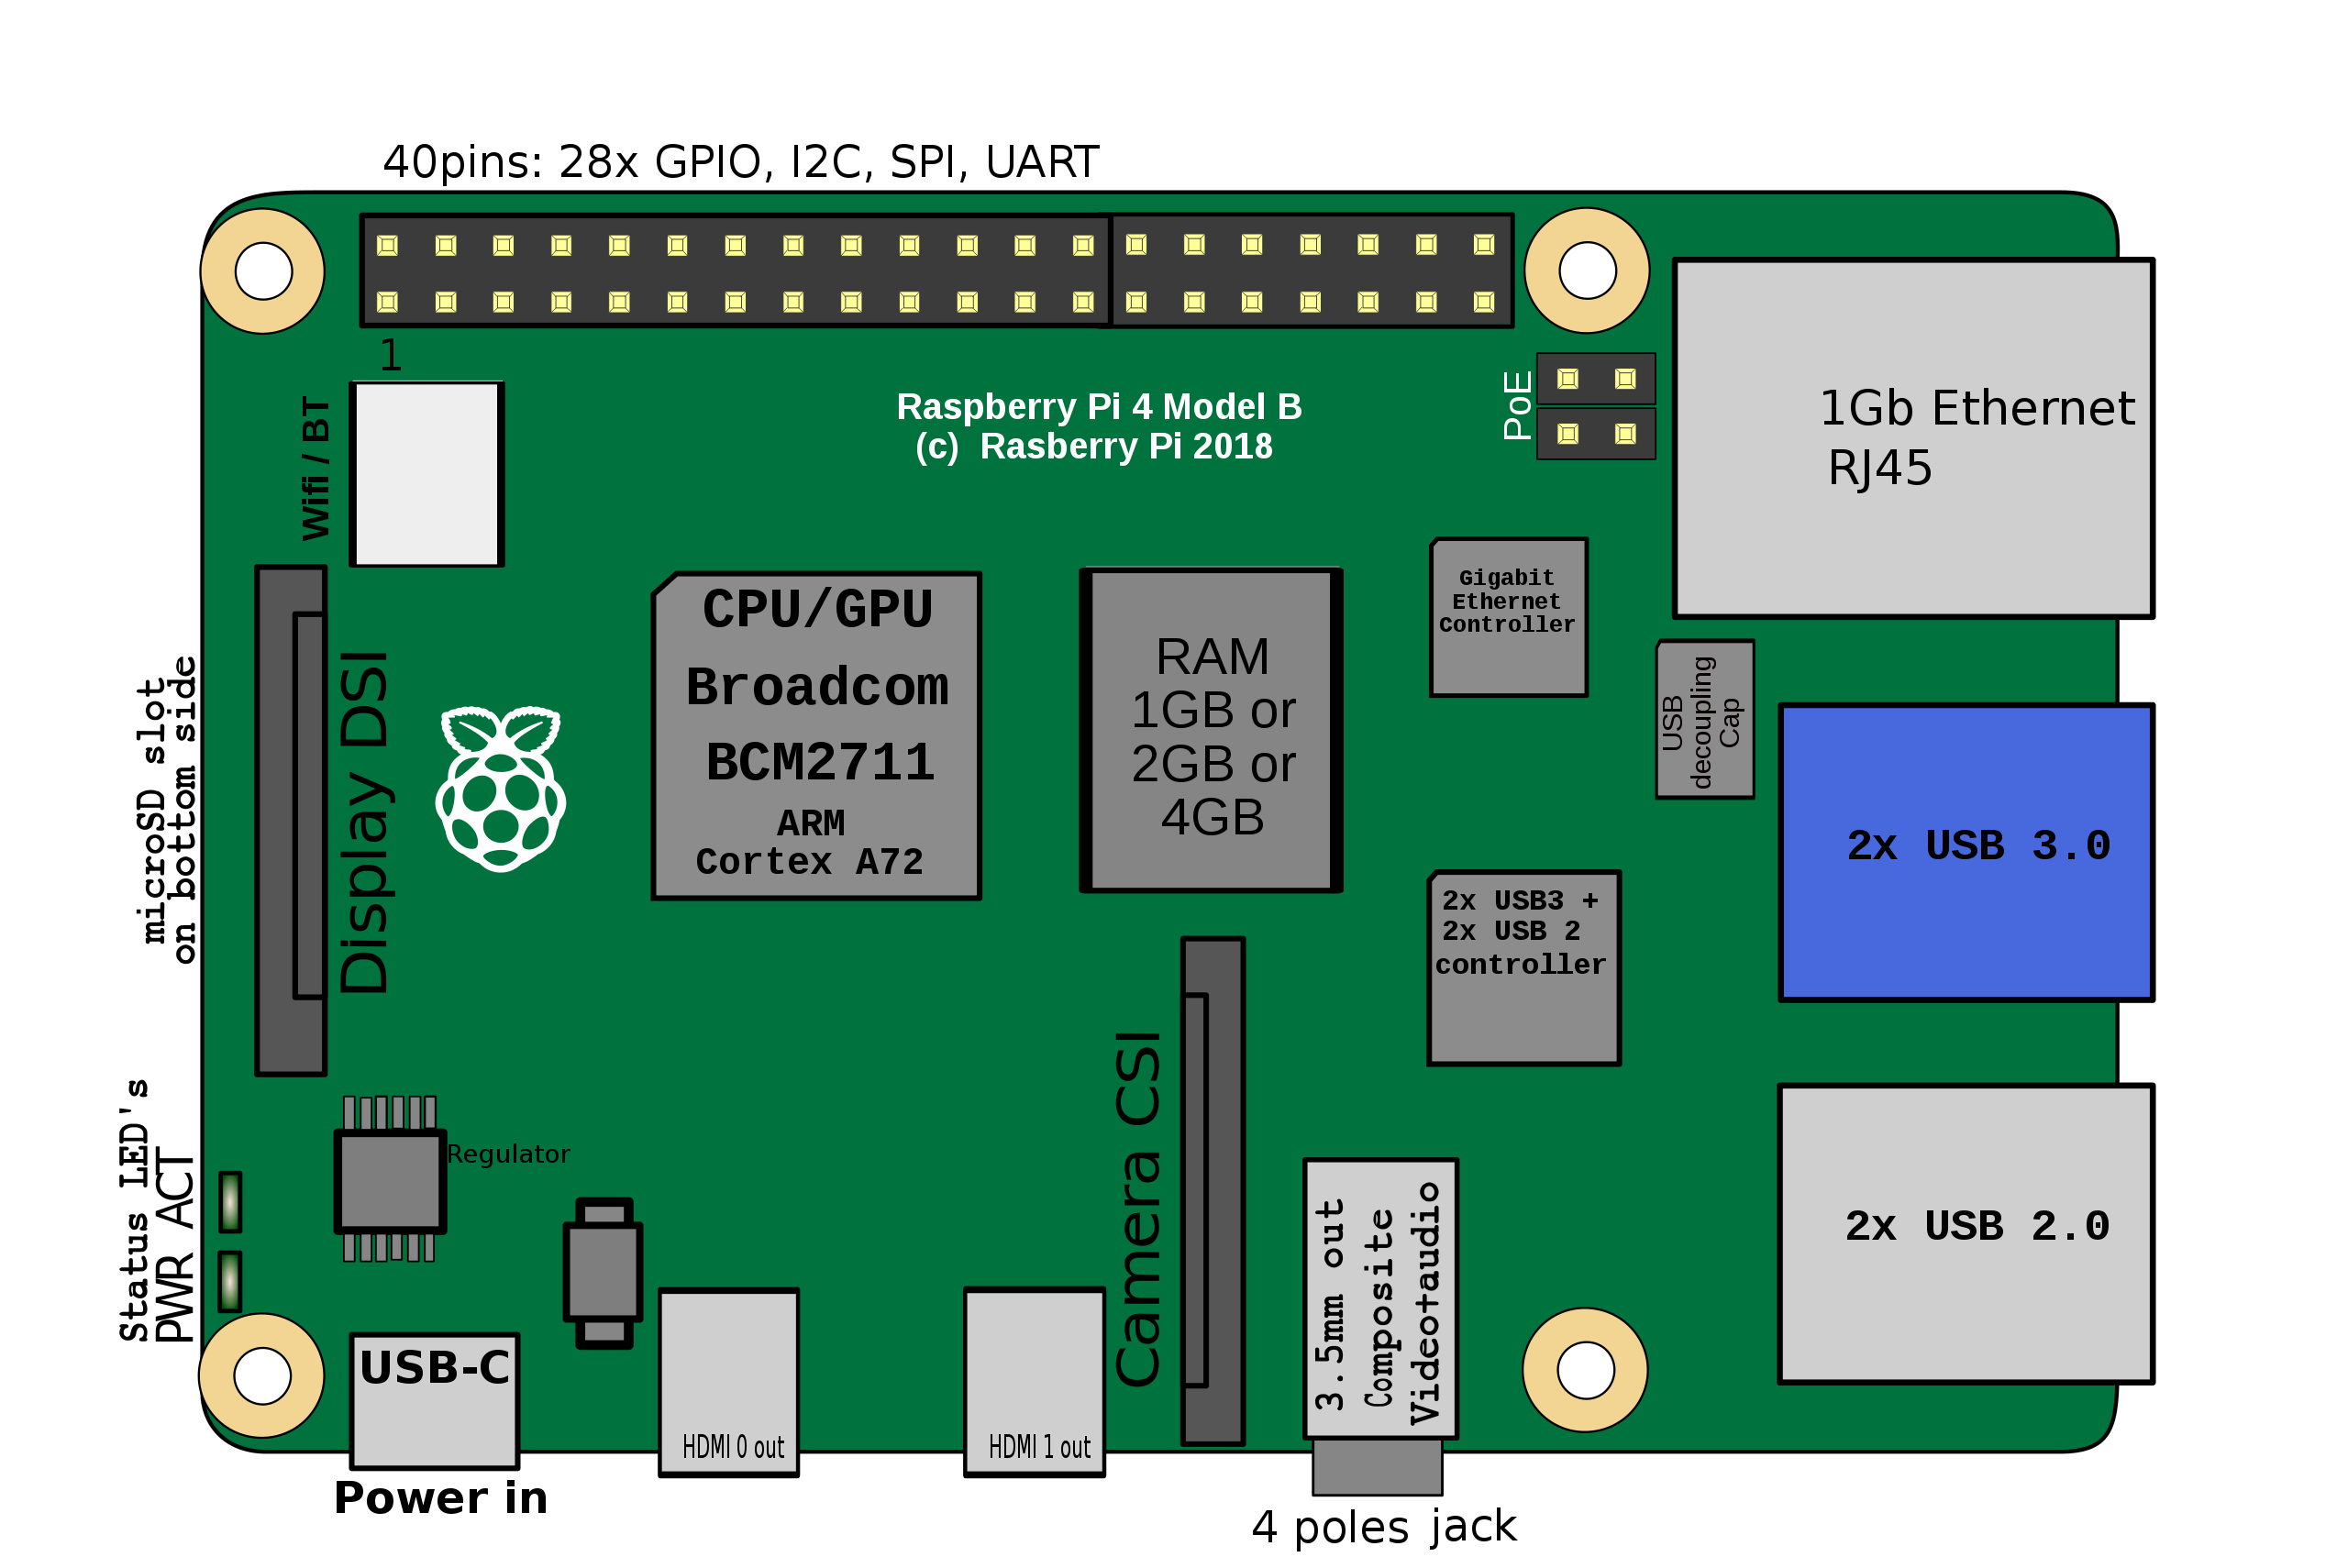
\includegraphics[width=10cm]{pics/2560px-RaspberryPi_4_Model_B.svg.png}
  \caption{Komponenten eines Raspberry Pi}
  \cite{RaspberryImage}
  \end{figure}


Auszeichnungsmerkmale des Raspberry Pi sind unter anderem die geringen Anschaffungskosten von ab 35 US-\$, sowie seine leistungsstarken Komponenten.\\
%\textbf{Bestandteile des Raspberry Pi} 
\begin{table}[H]
  \centering
  \caption{Übersicht der Komponenten des Raspberry Pi \cite{RaspySpecs}}
  \label{Komponenten des Raspberry Pi}
    \begin{adjustbox}{width=\textwidth}
      \begin{tabular}{lll}
      \hline
      \textbf{Komponente}                    & \textbf{Spezifikation}                                                    & \textbf{Besonderheiten}                    \\ \hline
      \multicolumn{1}{l|}{\textbf{Prozessor}} &
        \begin{tabular}[c]{@{}l@{}}Broadcom BCM2711\\ - Quad Core Prozessor @ 1.5GHz\end{tabular} &
        \begin{tabular}[c]{@{}l@{}}ARM Architektur\\ 64-Bit SoC\end{tabular} \\ \hline
      \multicolumn{1}{l|}{\textbf{RAM}}      & 1GB, 2GB, 4GB oder 8GB LPDDR4 SDRAM                                                          & Tatktung von 3200MHz                       \\ \hline
      \multicolumn{1}{l|}{\textbf{USB}}      & \begin{tabular}[c]{@{}l@{}}2 USB 3.0 Ports\\ 2 USB 2.0 Ports\end{tabular} &                                            \\ \hline
      \multicolumn{1}{l|}{\textbf{GPIO}}     & 40 Pin Header                                                             & Abwärtskompatibel mit Vorgängermodellen    \\ \hline
      \multicolumn{1}{l|}{\textbf{Display}}  & 2 micro-HDMI Ports                                                        & jeweils bis zu 4k60 möglich                \\ \hline
      \multicolumn{1}{l|}{\textbf{Speicher}} & Micro-SD Kartenslot                                                       & Speicherplatz für Betriebssystem und Daten \\ \hline
      \multicolumn{1}{l|}{\textbf{Strom}} &
        \begin{tabular}[c]{@{}l@{}}5V Eingang über USB-C Port\\ 5V Ausgang über GPIO-Header\end{tabular} &
        Anforderung an Stromquelle: mindestens 3A \\ \hline
      \end{tabular}
    \end{adjustbox}
  \end{table}
Der Raspberry Pi ist einer der am weitesten verbreiteten Ein-Platinen-Computer der Welt. Trotz der im Verhältnis zu größeren Systemen schwache Leistung im Jahr 2020 mehr als 7 Millionen mal verkauft worden. Daraus ergibt sich ein Marktanteil von allen PCs von 2.69\%.
Für ein ausgewogenes Verhältnis zwischen Kompaktheit und Leistung wurde auf einen Raspberry Pi 4 Model B in der Ausführung mit 4GB Arbeitsspeicher zurückgegriffen. Weiters waren die Anschaffungskosten von etwa 100\$ ein weiterer Grund für die Auswahl. \cite{RaspyMarketShare}

\textbf{Kernkomponenten des Raspberry Pi}\\
\textit{GPIO-Header}\\
Zu den Kernkomponenten, die den Raspberry Pi von anderen PC-Systemen unterscheidet, ist der GPIO-Header. GPIO steht für General Purpose Input / Output, und kann wörtlich zu Allzweckeingabe bzw. -ausgabe übersetzt werden. Sie bezeichnen selbst programmierbare Ein- und Ausgänge, die auf dem Raspberry Pi als angelötete Pins zur Verfügung stehen.
Der Raspberry kann über diese Schnittstellen digitale Signale von außen annehmen, sowie auch Signale abgeben.
Der Raspberry Pi in der Ausführung Model 4 B hat einen 40-köpfigen GPIO-Header in Form einer Stiftleiste mit zwei Reihen. Davon gibt es einige GPIOs mit bestimmten Zusatzfunktionen, wie I2C, SPI oder seriellen Schnittstellen. Weiters gibt es Pins, welche vom Raspberry eine +5V-Spannung, eine +3.3V Spannung, oder die Möglichkeit der Erdung liefern.\\ \\
\textit{GPIO-Belegung und elektrische Eigenschaften}\\ 
Grundsätzlich kann in elektronischen Systemen auf elektrische Eigenschaften zurückgegriffen werden, die beobachtet werden müssen. Oft sind diese Eigenschaften Grenzwerte des Systems, welche nicht überschritten werden dürfen. Wird dies ignoriert, kann das System nach Start beschädigt werden und im weiteren Verlauf Defekte aufweisen.
Die Eingangsspannung des Raspberry Pi beträgt zwar 5V, jedoch arbeitet der Prozessor selbst nur mit 3.3V. Daher haben auch die GPIOs nur 3.3V zur Verfügung. Dies gilt für die Ausgangsspannung, jedoch auch für die Eingangsspannung, da sonst der Chip des Raspberry Pi beschädigt werden kann. 
\begin{figure}
  \centering
  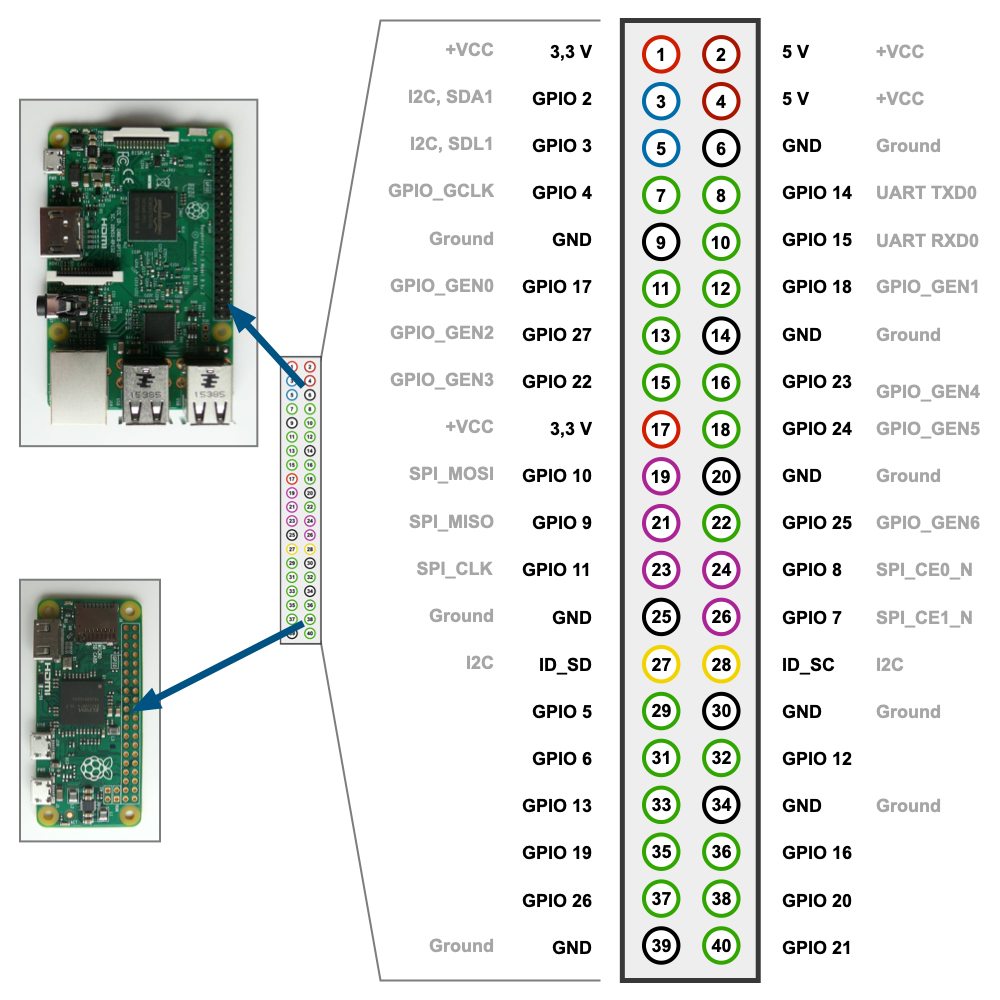
\includegraphics[width=10cm]{pics/GPIO.png}
  \caption{Belegung der GPIOs eines Raspberry Pi Model 4B oder Raspberry Pi Zero}
  \cite{GPIOLayout}
\end{figure}
GPIOs sind empfindliche Schnittstellen, denn sie können schon bei geringen Stromstärken Schaden nehmen. Theoretisch ist eine Stromstärke von 16mA (Milliampere) möglich, wobei diese nie benötigt wird, da die GPIOs schon mit einer Stromstärke von 0.5mA geschalten werden können. Um die Langlebigkeit des Raspberry Pi zu gewährleisten, sollten nie mehr als 8mA von einem GPIO abgegeben werden. 
Es gibt jedoch Ausnahmen, wie die +5V-Pins. Diese bieten für externe Schaltungen eine Spannung bis zu 5V an, sind jedoch ebenfalls bei der Stromentnahme begrenzt. Hier wird mit etwa 25mA pro 5V-Pin gerechnet. Sollte dies für eine Schaltung nicht ausreichen, kann auf externe Stromquellen zurückgegriffen werden, wie eine Stromversorgung über ein separates Netzteil mit USB-Anschluss, oder die Versorgung über einen der verfügbaren USB-Ports des Raspberry Pi selbst. 

\cite{GPIO}
\subsubsection{NFC-Leser}
\subsubsection{Numpad}
\subsubsection{Kamera}
Die Kamera ermöglicht dem Raspberry Pi, die Kennzeichen zu sehen und darauf die Kennzeichen zu erkennen. Dazu wird bei APERTA eine handelsübliche Webcam verwendet, die über einen der beiden USB 3.0 Ports am Raspberry angeschlossen wird.
Um genug Auflösung für die Kennzeichenerkennung zu gewährleisten, wurde auf eine Webcam zurückgegriffen, welche mit bis zu 1920 Pixeln mal 1080 Pixeln aufnehmen kann.
Alternativ wäre auch eine Raspberry Pi Camera möglich gewesen, jedoch wurde die aufgrund ihres kurzen Flachbandkabels nicht verwendet, um die Kamera auch in größere Entfernung vom Raspberry Pi nutzen zu können.
\begin{figure}[H]
  \centering
  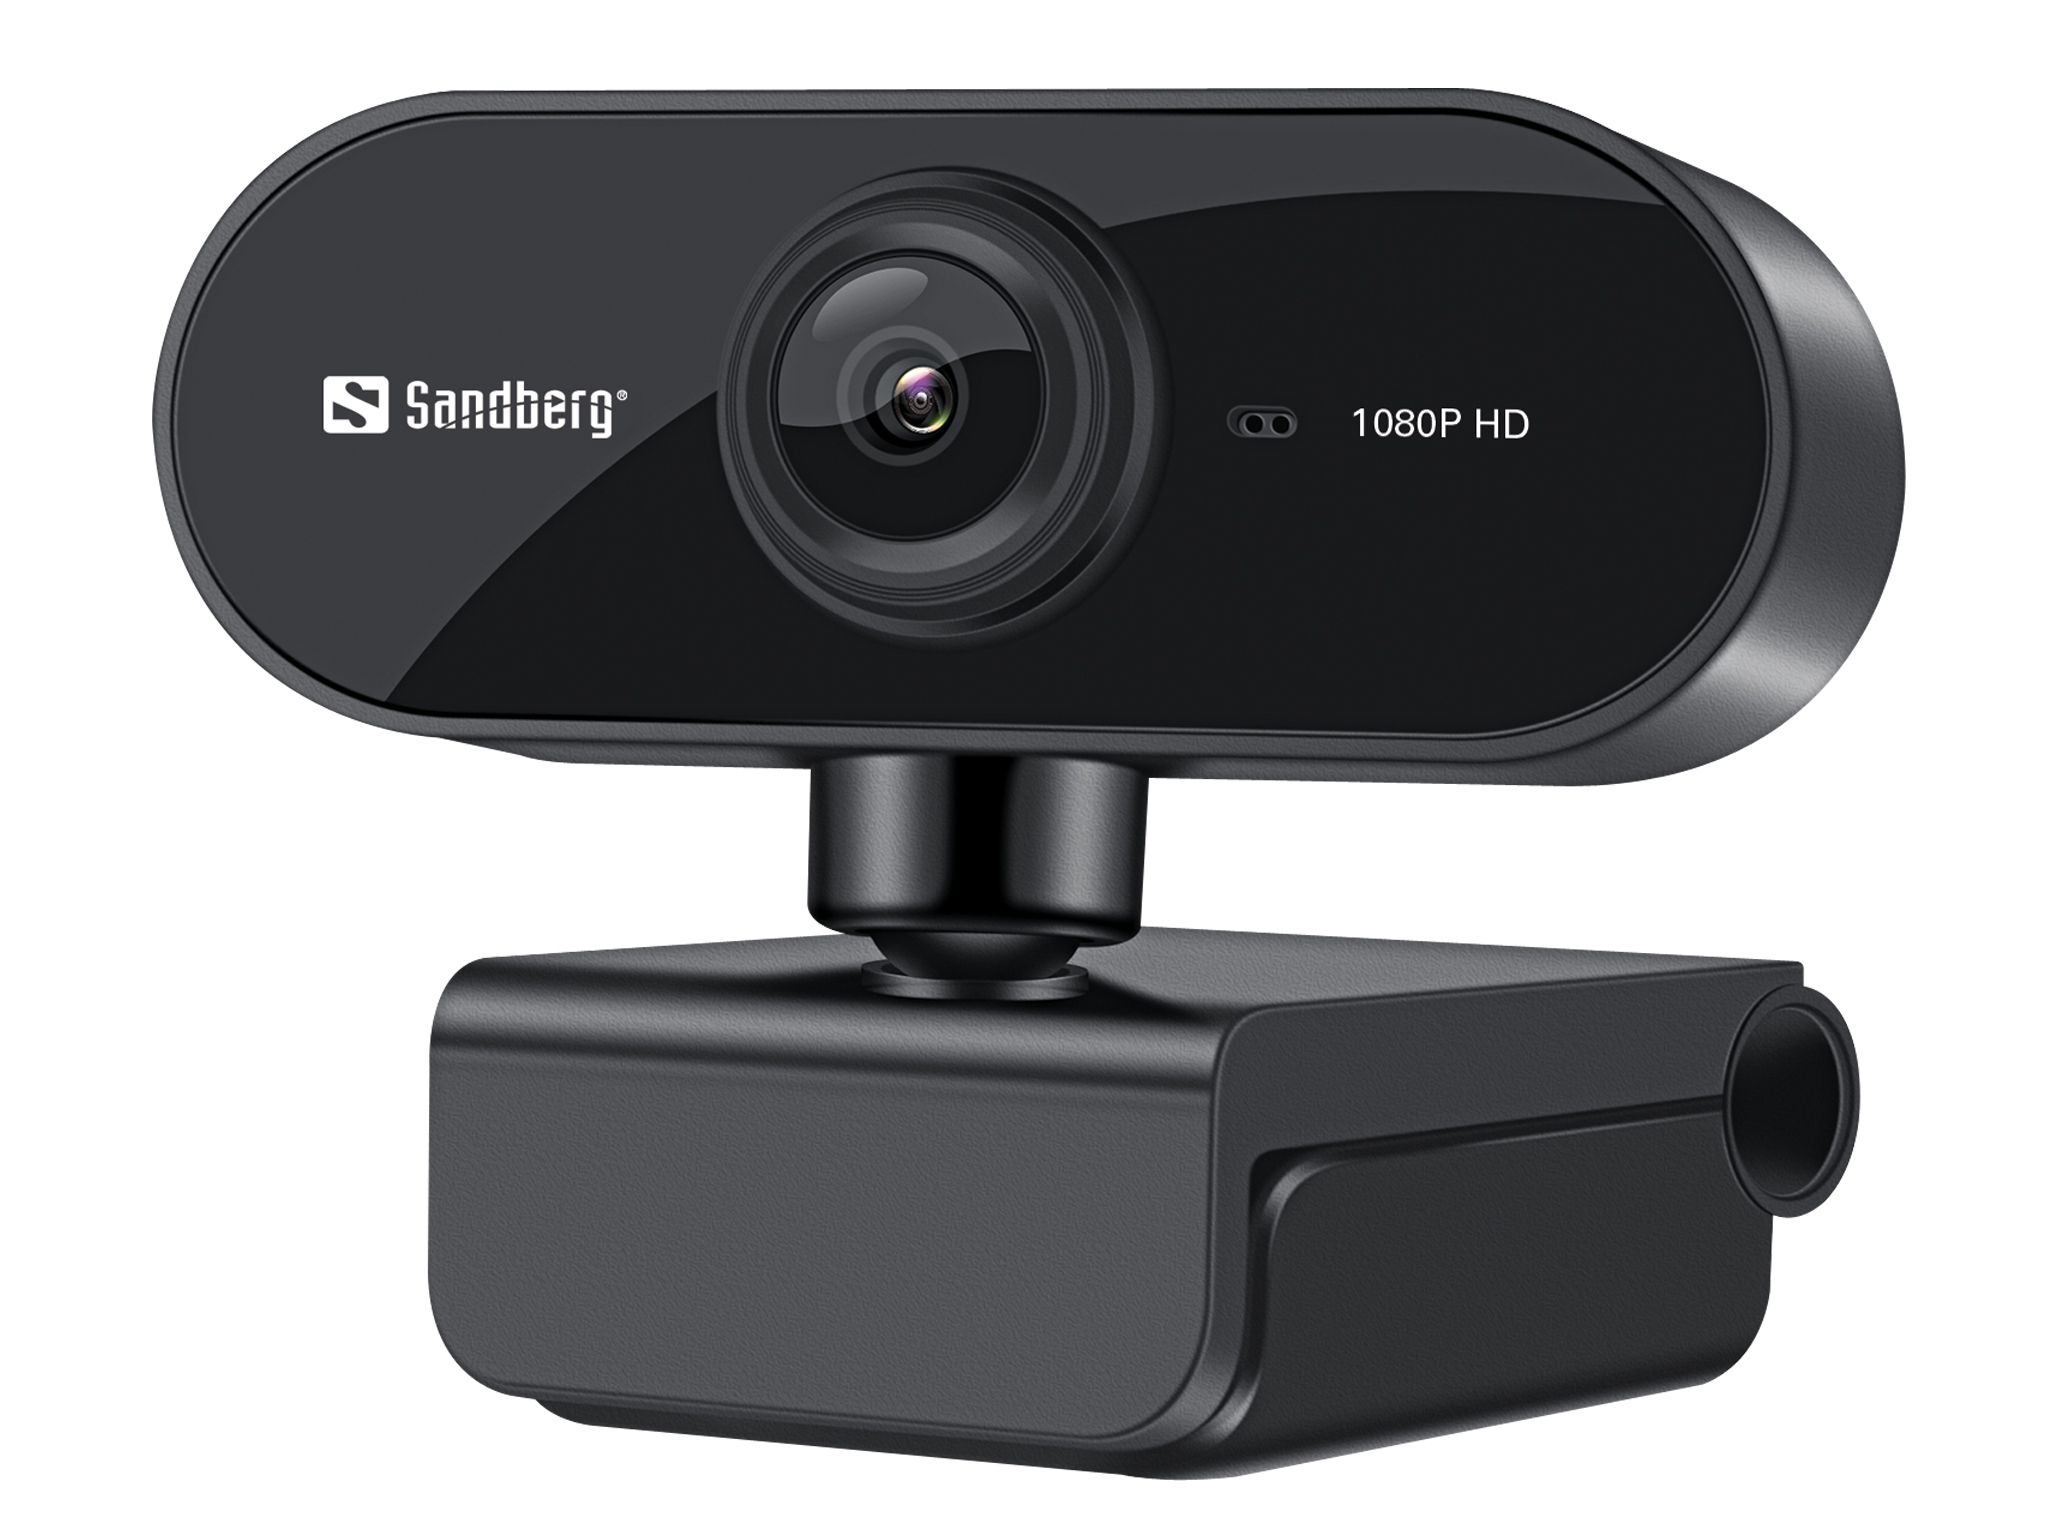
\includegraphics[width=8cm]{pics/Webcam.jpg}
  \caption{Webcam mit gleichen Spezifikationen}
  \cite{Webcam}
\end{figure}

\begin{figure}[H]
  \centering
  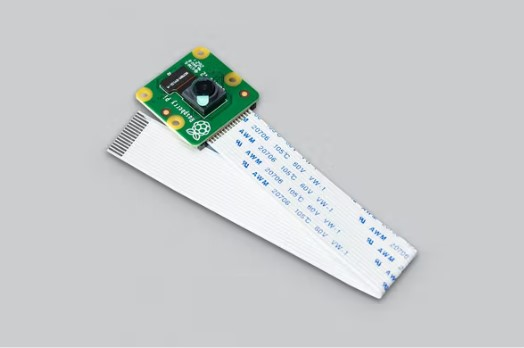
\includegraphics[width=8cm]{pics/RaspberryPiCameraModule2.jpg}
  \caption{Raspberry Pi Camera Module 2}
  \cite{PiCamera}
\end{figure}

\subsubsection{Display}

%\begin{figure}
  %\centering
 % 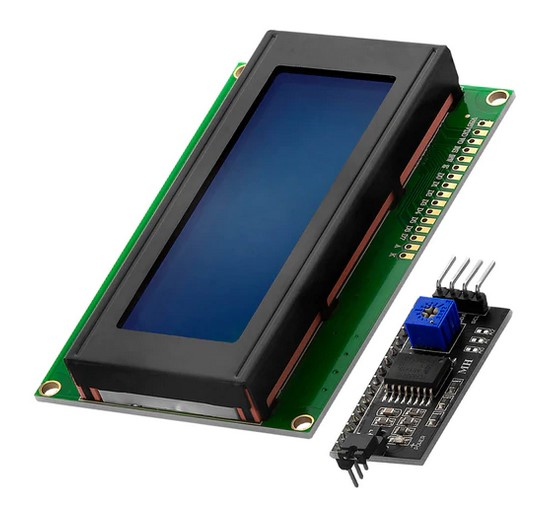
\includegraphics[width=8cm]{pics/RaspberryDisplay.jpg}
%\end{figure}

Um dem Nutzer vor der Garage mitzuteilen, was gerade geschieht, wird ein Display verwendet, auf dem mitgeteilt wird, ob die Kombination, welche auf dem Nummernfeld eingegeben wurde, korrekt ist, oder ob die NFC-Karte autorisiert ist.
Da auf diesem Display nur kurze Textausgaben angezeigt werden, fiel die Entscheidung auf ein LCD-Display gesetzt, welches in zwei Zeilen beschrieben werden kann. Dieses bat zudem weitere Vorteile wie die geringen Kosten von 9€ pro Stück, die Spannungsversorgung durch den Raspberry Pi selbst, sowie die einfache Möglichkeit, Text darauf auszugeben.
Im Lieferumfang des Displays war zudem ein I2C Serial Adapter, welcher durch seine 4 benötigen Ports um 8 Pins auf dem Raspberry Pi weniger benötigt, als das direkt angeschlossene Display. 
\begin{figure}[H]
  \centering
  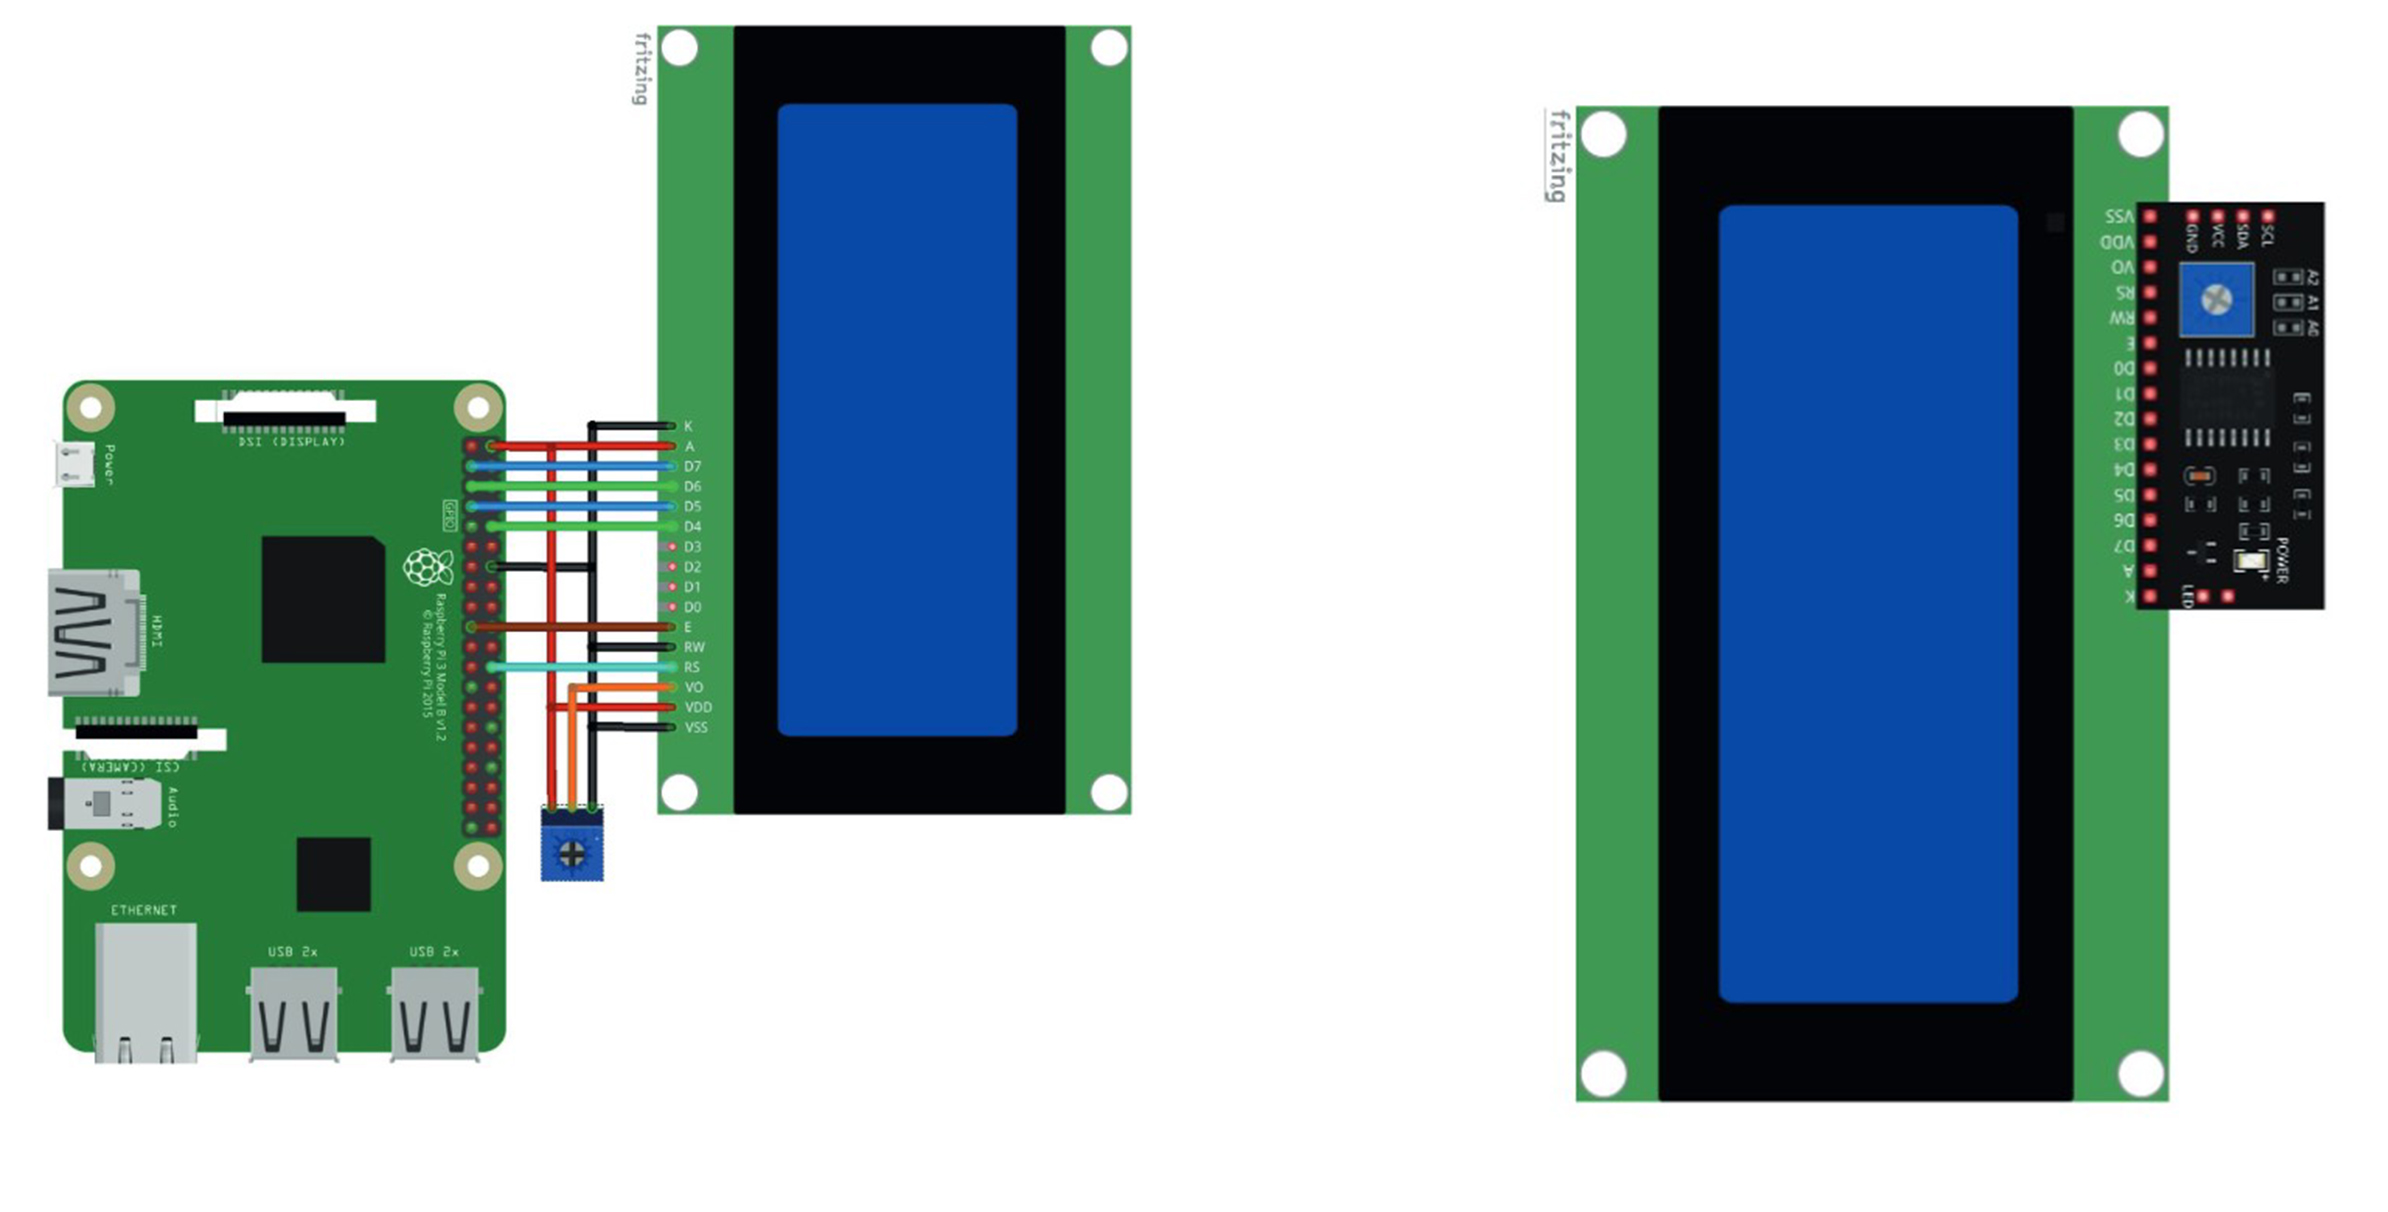
\includegraphics[width=15cm]{pics/DisplayComparison.jpg}
  \caption{Display direkt angeschlossen / Display über I2C Adapter angeschlossen}
\end{figure}
Die technischen Daten des Displays lauten:
\begin{itemize}
  \item 4 Zeilen zu je 20 Zeichen beschreibbar
  \item Blaue Hintergrundbeleuchtung
  \item 5V Versorgungsspannung
\end{itemize}
\cite{RaspberryDisplay}

 \subsubsection{Relais}
Handelsübliche Garagentore werden mit einer Spannung von 230 Volt betrieben. Der Raspberry Pi diese nicht direkt ansteuern, da diese Spannung die interne Elektronik des Pi zerstören würde. Dennoch ist es nötig, wie bei einem Schalter den Steuerstromkreis des Garagentores zu schließen, um den Öffnungsmechanismus zu aktivieren. Um dies zu erreichen, wird ein Relais verwendet, welches in den externen Stromkreis geschalten wird und wie eine Brücke den Stromkreis schließen kann. Ein Relais besteht aus einer Spule aus Draht und einem Metallkern. Wird Strom durch den Draht geschickt, wird der Kern magnetisiert. Ohne Strom verschwindet das Magnetfeld des Kerns wieder.

Das Relais ist ein Elektromagnet, welcher durch den Steuerkreis einen Eisenanker zu sich zieht und somit den Arbeitsstromkreis schließt. Der Arbeitsstromkreis kann unabhängig vom Steuerkreis aufgebaut sein und auch unterschiedliche Spannungen und Stromstärken besitzen. Wichtig ist nur, dass das richtige Relais für den Arbeitskreis verwendet wird. Im Fall diese Projektes wird ein Relais verwendet, welches für bis zu 250 Volt Gleichstrom des Arbeitskreises verwendet werden kann.
\cite{Relais}
\begin{figure}[H]
  \centering
  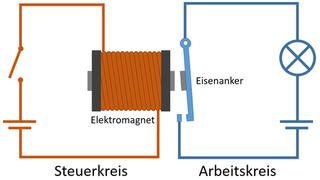
\includegraphics[width=8cm]{pics/Relais.png}
  \caption{Funktionsweise eines Relais als Schema}
  \cite{RelaisBild}
\end{figure}


\subsubsection{Steuerung der Hardware}
Um die Komponenten miteinander zu verbinden, war eine Programmiersprache notwendig, die mit den über GPIOs angeschlossenen Bauteilen kommunizieren kann. Dazu gab es eine Handvoll von Programmiersprachen, welche für die Entwicklung von Projekten mit dem Raspberry Pi in Frage kamen.

\begin{itemize}
  \item \textit{Scratch: }Scratch ist eine baukastenartige Programmiersprache, bei der Befehlsblöcke mithilfe der Maus aneinander angereiht werden. Entwickelt vom MIT Media Lab, richtet Scratch an Programmierneulinge und Kinder, da es sie unterstützen soll, programmieren zu lernen und Code lesen und verstehen zu können.
  \item \textit{Python: }Python zählt zu den meistverwendeten Programmiersprachen in Verbindung mit dem Raspberry Pi. Es zeichnet sich durch seine einsteigerfreundliche Syntax und die riesige Community aus, welche es ermöglicht, auf eine Vielzahl an Frameworks und Libraries zurückzugreifen. Python beschränkt sich dabei nicht auf einen bestimmten Einsatzbereich, sondern kann für die Entwicklung von graphischen Nutzeroberflächen, im Webdevelopment, zum Trainieren von Künstlichen Intelligenzen sowie für Automatisierung verwendet werden.
  \item \textit{JavaScript: } JavaScript ist nicht nur eine Erweiterung von HTML als Scripting Sprache, sondern viel mehr eine ganz eigenständige umfangreiche Programmiersprache. Sie wird meistens mit Webentwicklung in Verbindung gebracht, ist jedoch auch fähig, bereits bestehende Applikationen zu erweitern.
  \item \textit{Java: } Java ist eine der vielseitigsten Programmiersprachen, da sie erlaubt, unabhängig von Betriebssystem zu entwickeln, ohne den Code für jede Plattform verändern zu müssen. Mit mehr als 3 Milliarden Geräten, auf denen Java läuft, ist sie eine der meist verbreiteten Programmiersprachen.
  \item \textit{C: } C ist einer der stärksten Konkurrenten von Java. Raspbian OS, das Betriebssystem des Raspberry Pi, wurde beispielsweise in C geschrieben. C zeichnet sich durch einen klar strukturierten Programmierstil und die Möglichkeit, Arbeitsspeicher direkt anzusprechen, aus. Die Haupteinsatzgebiete von C sind die Entwicklung von Betriebssystemen und Compilern.
  \item \textit{C++: } Verglichen mit C, kann sich C++ mit objektorientierter Programmierung auszeichnen. Die Kombination aus prozeduraler und objektorientierterer Programmierung machen C++ zu einer Allzwecklösung, mit welcher von Betriebssystemen über Spiele bis hin zu Webbrowsern alles entwickelt werden kann.
  \item \textit{Perl: } Die Perl Org. hat mit Perl eine Sprache entwickelt, welche für fast jede Aufgabe, die mit C oder C++ Libraries zu tun hat, geeignet ist. Die große Auswahl an Libraries und Modulen sprechen trotz der geringen Bekanntheit für Perl, welche weiters für die Webentwicklung, Systemadministration, GUI-Entwicklung und vielem mehr verwendet werden kann.
  \item \textit{Erlang: } Erlang ist eine relativ unbekannte Sprache, da sie meist für Industrieapplikationen verwendet wird. Auszeichnungsmerkmale von Erlang sind beispielsweise die Fähigkeit, skalierbare Echtzeitsysteme zu entwickeln. Auch bei dezentralisierten Systemen ist Erlang eine gute Wahl, da das Programm bei Ausfall eines Rechners aus dem Cluster problemlos weiter arbeiten kann. Verwender sind unteranderem Banken und Telekommunikationsunternehmen.
\end{itemize}
\cite{RaspberryProgramming}
Durch die einfache Möglichkeit, mit den GPIOs zu arbeiten, sowie der einfach verständlichen Syntax, wurde Python verwendet. Das Team konnte somit zusätzlich auf bereits bestehende Kenntnisse aufbauen.